\documentclass{article}
\usepackage{float}
\usepackage{amsmath}
\usepackage{booktabs}
\usepackage{geometry}
  \geometry{
  a4paper,
  total={170mm, 257mm},
  left=20mm,
  top=20mm
  }
\title{Informe Técnico Demográfico}
\author{Miguel Lara}
\date{\today}
\usepackage{Sweave}
\begin{document}
\Sconcordance{concordance:informe_demografico.tex:informe_demografico.Rnw:1 14 1 1 0 %
2 1 1 19 6 1 1 7 14 0 1 2 19 1}



\maketitle

\section{Resumen de Indicadores por Continente}

Se presenta a continuación una tabla con los valores agregados y promedio de los principales indicadores demográficos por continente, correspondientes al año más reciente disponible en el dataset.

\begin{table}[!h]
\centering
\caption{Indicadores demográficos por continente (2024)}
\centering
\begin{tabular}[t]{llrrr}
\toprule
Continent & Total\_Population & Average\_Fertility & Average\_LifeExpectancy & Number\_of\_Countries\\
\midrule
Africa & 1.513.340.011 & 380 & 6678 & 54\\
Americas & 1.043.693.262 & 181 & 7629 & 35\\
Asia & 4.798.762.835 & 216 & 7535 & 49\\
Europe & 743.011.656 & 144 & 8020 & 42\\
Oceania & 45.226.118 & 283 & 6899 & 14\\
\bottomrule
\end{tabular}
\end{table}
\section{Relación entre Fertilidad y Esperanza de Vida media}

El siguiente gráfico muestra la relación entre la tasa de fertilidad (hijos por mujer) y la esperanza de vida (años) por país, agrupados por continente.

\begin{figure}[H]
\centering
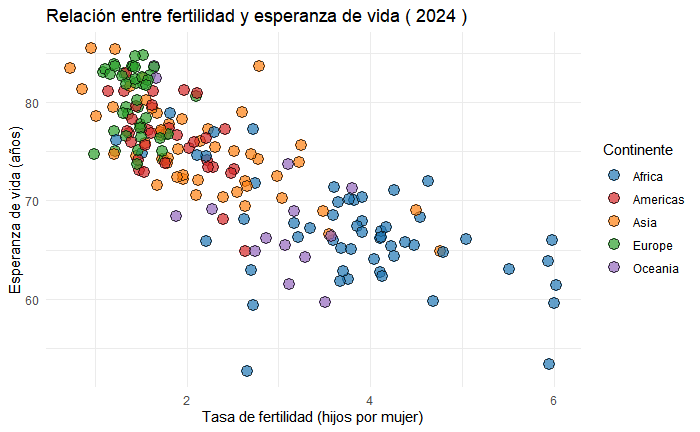
\includegraphics[width=0.7\textwidth]{fertility_life_expectancy.png}
\caption{Relación entre fertilidad y esperanza de vida}
\end{figure}

\section{Análisis}

Se observa una \textbf{relación inversa} clara entre fertilidad y esperanza de vida: los continentes con menor tasa de fertilidad parecen tender a tener una mayor esperanza de vida. \textbf{Europa} destaca por tener la fertilidad más baja (1,44 hijos por mujer) y la mayor esperanza de vida (80,2 años), mientras que \textbf{África} presenta la fertilidad más alta (3,80) y la esperanza de vida más baja (66,78 años), reflejando una etapa temprana de transición demográfica.

\textbf{Asia}, aunque tiene una fertilidad moderada (2,16), se posiciona en el gráfico con valores cercanos a cero en el eje de fertilidad y altos en el eje de esperanza de vida, lo que podría indicar que varios países asiáticos están en una fase avanzada de transición. \textbf{América} también muestra baja fertilidad (1,81) y alta esperanza de vida (76,29), mientras que \textbf{Oceanía} se ubica con fertilidad relativamente alta (2,83) y esperanza de vida intermedia (68,99), reflejando su diversidad interna.

Estos patrones permiten visualizar de forma clara las diferencias estructurales entre continentes en términos de salud, desarrollo y dinámica poblacional.

\end{document}
